% Basic Category Theory
% Tom Leinster <Tom.Leinster@ed.ac.uk>
% 
% Copyright (c) Tom Leinster 2014-2016
% 
% Chapter 2: Adjoints
% 

\chapter{Adjoints}
\label{ch:adj}


The slogan of Saunders Mac Lane's book \emph{Categories for the Working
  Mathematician} is:
% 
\begin{slogan}
Adjoint functors arise everywhere.
\end{slogan}
% 
We will see the truth of this, meeting examples of adjoint functors from
diverse parts of mathematics.  To complement the understanding provided by
examples, we will approach the theory of adjoints from three different
directions, each of which carries its own intuition.  Then we will prove
that the three approaches are equivalent.

Understanding adjointness gives you a valuable addition to your
mathematical toolkit.  Most professional pure mathematicians know what
categories and functors are, but far fewer know about adjoints.  More
should: adjoint functors are both common and easy, and knowing about
adjoints helps you to spot patterns in the mathematical landscape.



\section{Definition and examples}
\label{sec:adj-basics}


Consider a pair of functors in opposite directions, $F\from \cat{A} \to
\cat{B}$ and $G\from \cat{B} \to \cat{A}$.  Roughly speaking, $F$ is said
to be left adjoint to $G$ if, whenever $A \in \cat{A}$ and $B \in \cat{B}$,
maps $F(A) \to B$ are essentially the same thing as maps $A \to G(B)$.

\begin{defn}    
\label{defn:adjn}
Let $\oppairi{\cat{A}}{\cat{B}}{F}{G}$ be categories and functors.  We say
that $F$ is \demph{left adjoint}%
%
\index{adjunction}
%
to $G$, and $G$ is \demph{right adjoint} to $F$, and write $F \ladj G$,%
%
\ntn{ladj}
%
 if
% 
\begin{equation}        
\label{eq:adjn}
\cat{B}(F(A), B)
\iso
\cat{A}(A, G(B))
\end{equation}
% 
naturally in $A \in \cat{A}$ and $B \in \cat{B}$.  The meaning of
`naturally' is defined below.  An \demph{adjunction} between $F$ and $G$ is
a choice of natural isomorphism~\eqref{eq:adjn}.
\end{defn}

`Naturally in $A \in \cat{A}$ and $B \in \cat{B}$' means that there is a
specified bijection~\eqref{eq:adjn} for each $A \in \cat{A}$ and $B \in
\cat{B}$, and that it satisfies a naturality axiom.  To state it, we need
some notation.  Given objects $A \in \cat{A}$ and $B \in \cat{B}$, the
correspondence~\eqref{eq:adjn} between maps $F(A) \to B$ and $A \to G(B)$
is denoted by a horizontal bar,%
%
\ntn{adj-bar}
%
in both directions:
\[
\begin{array}{ccc}
\Bigl(F(A) \toby{g} B\Bigr)             &
\mapsto	&
\Bigl(A \toby{\bar{g}} G(B)\Bigr),	\\
\Bigl(F(A) \toby{\bar{f}} B\Bigr)	&
\mapsfrom	&
\Bigl(A \toby{f} G(B)\Bigr).
\end{array}
\]
So $\bar{\bar{f}} = f$ and $\bar{\bar{g}} = g$.  We call
$\bar{f}$ the \demph{transpose}%
%
\index{transpose}
%
of $f$, and similarly for $g$.  The naturality%
%
\index{adjunction!naturality axiom for}
%
axiom has two parts:
% 
\begin{equation}        
\label{eq:adj-nat-a}
\ovln{\Bigl(F(A) \toby{g} B \toby{q} B'\Bigr)}
\quad
=
\quad
\Bigl(A \toby{\bar{g}} G(B) \toby{G(q)} G(B')\Bigr)
\end{equation}
% 
(that is, $\ovln{q \of g} = G(q) \of \bar{g}$) for all $g$ and $q$, and 
% 
\begin{equation}        
\label{eq:adj-nat-b}
\ovln{\Bigl(A' \toby{p} A \toby{f} G(B)\Bigr)}
\quad
=
\quad
\Bigl(F(A') \toby{F(p)} F(A) \toby{\bar{f}} B\Bigr)
\end{equation}
% 
for all $p$ and $f$.  It makes no difference whether we put the long bar
over the left or the right of these equations, since bar is self-inverse.


\begin{remarks} 
\label{rmks:adjts}
\begin{enumerate}[(b)]
\item           
\label{rmk:adjts:nat}
The naturality axiom might seem ad hoc, but we will see in
Chapter~\ref{ch:rep} that it simply says that two particular functors are
naturally isomorphic.  In this section, we ignore the naturality axiom
altogether, trusting that it embodies our usual intuitive idea of
naturality: something defined without making any arbitrary choices.

\item 
The naturality axiom implies that from each array of maps
\[
A_0 \to \cdots \to A_n,
\quad
F(A_n) \to B_0,
\quad
B_0 \to \cdots \to B_m,
\]
it is possible to construct exactly one%
%
\index{uniqueness!constructions@of constructions}
%
map
\[
A_0 \to G(B_m).
\]
Compare the comments on the definitions of category, functor and natural
transformation (Remarks~\ref{rmks:defn-cat}\bref{rmk:defn-cat:loosely},
\ref{rmks:defn-ftr}\bref{rmk:defn-ftr:loosely},
and~\ref{rmks:defn-nt}\bref{rmk:defn-nt:loosely}).

\item   
\label{rmk:Lie-ass}
Not only do adjoint functors arise everywhere; better, whenever you see a
pair of functors $\cat{A}\oppairu \cat{B}$, there is an excellent chance
that they are adjoint (one way round or the other).

For example, suppose you get talking to a mathematician who tells you that
her work involves Lie%
%
\index{algebra!associative|(}%
\index{associative algebra|(}%
\index{Lie algebra|(}
%
algebras and associative algebras.  You try to object
that you don't know what either of those things is, but she carries on
talking anyway, explaining that there's a way of turning any Lie algebra
into an associative algebra, and also a way of turning any associative
algebra into a Lie algebra.  At this point, even without knowing what she's
talking about, you should bet her that one process is adjoint to the other.
This almost always works.

\item   
\label{rmks:adjts:uniqueness}
A given functor $G$ may or may not have a left adjoint, but if it does, it is
unique%
%
\index{adjunction!uniqueness of adjoints}
%
up to isomorphism, so we may speak of `\emph{the} left adjoint of $G$'.
The same goes for right adjoints.  We prove this later
(Example~\ref{eg:yon-adjts-unique}).

You might ask `what do we gain from knowing that two functors are adjoint?'
The uniqueness is a crucial part of the answer.  Let us return to the
example of~\bref{rmk:Lie-ass}.  It would take you only a few minutes to
learn what Lie algebras are, what associative algebras are, and what the
standard functor $G$ is that turns an associative algebra into a Lie
algebra.  What about the functor $F$ in the opposite direction?  The
description of $F$ that you will find in most algebra books (under
`universal%
%
\index{universal!enveloping algebra} 
%
enveloping algebra') takes much longer to understand.  However, you can
bypass that process completely, just by knowing that $F$ is the left
adjoint of $G$.  Since $G$ can have only \emph{one} left adjoint, this
characterizes $F$ completely.  In a sense, it tells you all you need to
know.%
%
\index{algebra!associative|)}%
\index{associative algebra|)}%
\index{Lie algebra|)}
%
\end{enumerate}
\end{remarks}


\begin{examples}[Algebra: free $\ladj$ forgetful]      
\label{egs:adjns-alg}
%
\index{adjunction!free--forgetful|(}
%
Forgetful%
%
\index{functor!forgetful!left adjoint to}
%
functors between categories of algebraic structures usually have left
adjoints.  For instance:
% 
\begin{enumerate}[(b)]
\item   
\label{eg:adjns-alg:vs}
Let $k$ be a field.  There is an adjunction
\[
\adjn{\Vect_k}{\Set,}{F}{U}
%
\index{vector space!free}
%
\]
where $U$ is the forgetful functor of
Example~\ref{egs:forgetful-functors}\bref{eg:forgetful-ring-vs} and $F$ is
the free functor of Example~\ref{egs:free-functors}\bref{eg:free-vs}.
Adjointness says that given a set $S$ and a vector space $V$, a linear map
$F(S) \to V$ is essentially the same thing as a function $S \to U(V)$.

We saw this in Example~\ref{eg:univ-basis}, but let us now check it in
detail.

Fix a set $S$ and a vector space $V$.  Given a linear map $g\from F(S) \to
V$, we may define a map of sets $\bar{g}\from S \to U(V)$ by $\bar{g}(s) =
g(s)$ for all $s \in S$.  This gives a function
\[
\begin{array}{ccc}
\Vect_k(F(S), V)        &\to            &\Set(S, U(V))  \\
g                       &\mapsto        &\bar{g}.
\end{array}
\]
In the other direction, given a map of sets $f\from S \to U(V)$, we may
define a linear map $\bar{f}\from F(S) \to V$ by $\bar{f} \bigl( \sum_{s
  \in S} \lambda_s s \bigr) = \sum_{s \in S} \lambda_s f(s)$ for all formal
linear combinations $\sum \lambda_s s \in F(S)$.  This gives a function
\[
\begin{array}{ccc}
\Set(S, U(V))  &\to            &\Vect_k(F(S), V)       \\
f              &\mapsto        &\bar{f}.
\end{array}
\]
These two functions `bar' are mutually inverse: for any linear map $g\from
F(S) \to V$, we have
\[
\bar{\bar{g}} \Biggl( \sum_{s \in S} \lambda_s s \Biggr)
=
\sum_{s \in S} \lambda_s \bar{g}(s)
=
\sum_{s \in S} \lambda_s g(s)
=
g \Biggl( \sum_{s \in S} \lambda_s s \Biggr)
\]
for all $\sum \lambda_s s \in F(S)$, so $\bar{\bar{g}} = g$, and for any
map of sets $f\from S \to U(V)$, we have
\[
\bar{\bar{f}}(s)
=
\bar{f}(s)
=
f(s)
\]
for all $s \in S$, so $\bar{\bar{f}} = f$.  We therefore have a canonical
bijection between $\Vect_k(F(S), V)$ and $\Set(S, U(V))$ for each $S \in
\Set$ and $V \in \Vect_k$, as required.

Here we have been careful to distinguish between the vector space $V$ and
its underlying set $U(V)$.  Very often, though, in category theory as in
mathematics at large, the symbol for a forgetful functor is omitted.  In
this example, that would mean dropping the $U$ and leaving the reader to
figure out whether each occurrence of $V$ is intended to denote the vector
space itself or its underlying set.  We will soon start using such
notational shortcuts ourselves.

\item   
\label{egs:adjns-alg:gp}
In the same way, there is an adjunction
\[
\adjn{\Grp}{\Set}{F}{U}
%
\index{group!free}
%
\]
where $F$ and $U$ are the free and forgetful functors of
Examples~\ref{egs:forgetful-functors}\bref{eg:forgetful-groups}
and~\ref{egs:free-functors}\bref{eg:free-group}.  

The free group functor is tricky to construct explicitly.  In
Chapter~\ref{ch:arl}, we will prove a result (the general adjoint functor
theorem) guaranteeing that $U$ and many functors like it all have left
adjoints.  To some extent, this removes the need to construct $F$
explicitly, as observed in
Remark~\ref{rmks:adjts}\bref{rmks:adjts:uniqueness}.  The point can be
overstated: for a group theorist, the more descriptions of free groups that
are available, the better.  Explicit%
%
\index{explicit description}
%
constructions really can be useful.  But it is an important general
principle that forgetful functors of this type always have left adjoints.

\item 
There is an adjunction
\[
\adjn{\Ab}{\Grp}{F}{U}
\]
where $U$ is the inclusion functor of
Example~\ref{egs:forgetful-functors}\bref{eg:forgetful-ab}.  If $G$ is a
group then $F(G)$ is the \demph{abelianization}%
%
\index{abelianization}%
\index{group!abelianization of}
%
$\abel{G}$%
%
\ntn{abel}
%
of $G$.  This is an abelian quotient group of $G$, with the property that
every map from $G$ to an abelian group factorizes uniquely through
$\abel{G}$:
\[
\xymatrix{
G \ar[r]^-\eta \ar[dr]_{\forall\phi}	&
\abel{G} \ar@{.>}[d]^{\exists!\bar{\phi}}	\\
&
\forall A.
}
\]
Here $\eta$ is the natural map from $G$ to its quotient $\abel{G}$, and $A$
is any abelian group.  (We have adopted the abuse of notation advertised in
example~\bref{eg:adjns-alg:vs}, omitting the symbol $U$ at several places
in this diagram.)  The bijection
\[
\Ab(\abel{G}, A) \iso \Grp(G, U(A))
\]
is given in the left-to-right direction by $\psi \mapsto \psi\of\eta$, and
in the right-to-left direction by $\phi \mapsto \bar{\phi}$.

(To construct $\abel{G}$, let $G'$ be the smallest normal subgroup of $G$
containing $xyx^{-1}y^{-1}$ for all $x, y \in G$, and put $\abel{G} =
G/G'$.  The kernel of any homomorphism from $G$ to an abelian group
contains $G'$, and the universal property follows.)

\item   
\label{eg:adjns-alg:gp-mon}
There are adjunctions
\[
\xymatrix{
\Grp \ar[d]|{U\vphantom{gl'}}	\\
\Mon \ar@<3ex>[u]^F_\ladj \ar@<-3ex>[u]_R^\ladj
}
%
\index{group!free on monoid}%
\index{monoid!free group on}
\]
between the categories of groups and monoids.  The middle functor $U$ is
inclusion.  The left adjoint $F$ is, again, tricky to describe explicitly.
Informally, $F(M)$ is obtained from $M$ by throwing in an inverse to every
element.  (For example, if $M$ is the additive monoid of natural numbers
then $F(M)$ is the group of integers.)  Again, the general adjoint functor
theorem (Theorem~\ref{thm:gaft}) guarantees the existence of this adjoint.

This example is unusual in that forgetful functors do not usually have
\emph{right} adjoints.  Here, given a monoid $M$, the group $R(M)$ is the
submonoid of $M$ consisting of all the invertible elements.

The category $\Grp$ is both a \demph{reflective}%
%
\index{subcategory!reflective}%
\index{reflective}
%
and a \demph{coreflective}%
%
\index{coreflective}
%
subcategory of $\Mon$.  This means, by definition, that the inclusion
functor $\Grp \incl \Mon$ has both a left and a right adjoint.  The
previous example tells us that $\Ab$ is a reflective subcategory of $\Grp$.

\item   
\label{egs:adjns-alg:fields}
Let $\Field$%
%
\ntn{Field}
%
be the category of fields,%
%
\index{field}
%
with ring homomorphisms as the maps.  The forgetful functor $\Field \to \Set$
does \emph{not} have a left adjoint.  (For a proof, see
Example~\ref{eg:no-free-field}.)  The theory of fields is unlike the
theories of groups, rings, and so on, because the operation $x \mapsto
x^{-1}$ is not defined for \emph{all} $x$ (only for $x \neq 0$).
%
\index{adjunction!free--forgetful|)}
%
\end{enumerate}
\end{examples}

\begin{remark}  
\label{rmk:alg-thy}
At several points in this book, we make contact with the idea of an
\demph{algebraic%
%
\index{algebraic theory}
%
theory}.  You already know several examples: the theory of groups is an
algebraic theory, as are the theory of rings, the theory of vector spaces
over $\reals$, the theory of vector spaces over $\complexes$, the theory of
monoids, and (rather trivially) the theory of sets.  After reading the
description below, you might conclude that the word `theory' is overly
grand, and that `definition' would be more appropriate.  Nevertheless, this
is the established usage.

We will not need to define `algebraic theory' formally, but it will be
important to have the general idea.  Let us begin by considering the theory
of groups.

A group can be defined as a set $X$ equipped with a function $\cdot \from X
\times X \to X$ (multiplication), another function $\blank^{-1}\from X \to
X$ (inverse), and an element $e \in X$ (the identity), satisfying a
familiar list of equations.  More systematically, the three pieces of
structure on $X$ can be seen as maps of sets
\[
\cdot\from X^2 \to X, 
\qquad
\blank^{-1}\from X^1 \to X,
\qquad
e\from X^0 \to X,
\]
where in the last case, $X^0$ is the one-element set $1$ and we are using
the observation that a map $1 \to X$ of sets is essentially the same thing
as an element of $X$.

(You may be more familiar with a definition of group in which only the
multiplication and perhaps the identity are specified as pieces of
\emph{structure}, with the existence of inverses required as a
\emph{property}.  In that approach, the definition is swiftly followed by a
lemma on uniqueness of inverses, guaranteeing that it makes sense to speak
of \emph{the} inverse of an element.  The two approaches are equivalent,
but for many purposes, it is better to frame the definition in the way
described in the previous paragraph.) 

An algebraic theory consists of two things: first, a collection of
operations, each with a specified arity%
%
\index{arity} 
%
(number of inputs), and second, a collection of equations.  For example,
the theory of groups has one operation of arity $2$, one of arity $1$, and
one of arity $0$.  An \demph{algebra}%
%
\index{algebra!algebraic theory@for algebraic theory}
%
or \demph{model}%
%
\index{model}
%
for an algebraic theory consists of a set $X$ together with a specified map
$X^n \to X$ for each operation of arity $n$, such that the equations hold
everywhere.  For example, an algebra for the theory of groups is exactly a
group.

A more subtle example is the theory of vector spaces over $\reals$.  This is
an algebraic theory with, among other things, an infinite number of
operations of arity $1$: for each $\lambda \in \reals$, we have the
operation $\lambda \cdot \dashbk\from X \to X$ of scalar multiplication by
$\lambda$ (for any vector space $X$).  There is nothing special about the
field $\reals$ here; the only point is that it was chosen in advance.  The
theory of vector spaces over $\reals$ is different from the theory of
vector spaces over $\complexes$, because they have different operations of
arity $1$.

In a nutshell, the main property of algebras for an algebraic theory is
that the operations are defined everywhere on the set, and the equations
hold everywhere too.  For example, \emph{every} element of a group has a
specified inverse, and \emph{every} element $x$ satisfies the equation $x
\cdot x^{-1} = 1$.  This is why the theories of groups, rings, and so on,
are algebraic theories, but the theory of fields is not.
\end{remark}

\begin{example}
\label{eg:adjn:spaces}
There are adjunctions
\[
\xymatrix{
\Tp \ar[d]|{U\vphantom{gl'}}	\\
\Set \ar@<3ex>[u]^D_\ladj \ar@<-3ex>[u]_I^\ladj
}
\]
where $U$ sends a space to its set of points, $D$ equips a set with the
discrete%
%
\index{topological space!discrete}
%
topology, and $I$ equips a set with the indiscrete%
%
\index{topological space!indiscrete}%
\index{indiscrete space}
%
topology.
\end{example}

\begin{example}
\label{eg:adjn:cc}
Given sets $A$ and $B$, we can form their (cartesian) product%
%
\index{set!category of sets!products in}
%
$A \times B$.  We can also form the set $B^A$%
%
\index{set!functions@of functions}%
\index{function!set of functions}
%
of functions from $A$ to $B$.  This is the same as the set $\Set(A, B)$,
but we tend to use the notation $B^A$ when we want to emphasize that it is
an object of the same category as $A$ and $B$.

Now fix a set $B$.  Taking the product with $B$ defines a functor
\[
\begin{array}{cccc}
\dashbk \times B\from	&\Set	&\to	&\Set   \\
			&A	&\mapsto&A \times B.
\end{array}
\]
(Here we are using the blank notation introduced in
Example~\ref{eg:fns-on-vs}.)  There is also a functor
\[
\begin{array}{cccc}
(\dashbk)^B\from	&\Set	&\to	&\Set   \\
			&C	&\mapsto&C^B.
\end{array}
\]
Moreover, there is a canonical bijection
\[
\Set(A \times B, C)
\iso 
\Set(A, C^B)
\]
for any sets $A$ and $C$.  It is defined by simply changing the
punctuation: given a map $g\from A \times B \to C$, define $\bar{g}\from A
\to C^B$ by
\[
(\bar{g}(a))(b) = g(a, b)
\]
($a \in A$, $b \in B$), and in the other direction, given $f\from A \to
C^B$, define $\bar{f}\from A \times B \to C$ by
\[
\bar{f}(a, b) = (f(a))(b)
\]
($a \in A$, $b \in B$).  Figure~\ref{fig:curry} shows an example with $A =
B = C = \reals$.  By slicing up the surface as shown, a map $\reals^2 \to
\reals$ can be seen as a map from $\reals$ to $\{\text{maps } \reals \to
\reals\}$.  

Putting all this together, we obtain an adjunction
\[
\adjn{\Set}{\Set}{\dashbk\times B}{(\dashbk)^B}
\]
for every set $B$.
\end{example}

\begin{figure}
\centering
\setlength{\unitlength}{1em}%
\begin{picture}(10,11.5)(-5,-.8)
\cell{0}{0}{b}{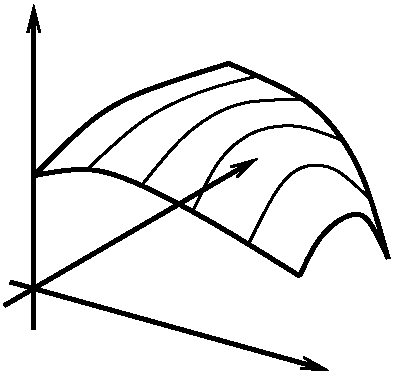
\includegraphics[width=10em]{curry}}
\cell{3.8}{-0.2}{c}{A}
\cell{2.2}{5.8}{c}{B}
\cell{-4.1}{10.1}{c}{C}
\end{picture}
\caption{In $\Set$, a map $A \times B \to C$ can be seen as a way of
  assigning to each element of $A$ a map $B \to C$.}
\label{fig:curry}  
\end{figure}

\begin{defn}    
\label{defn:init-term}
Let $\cat{A}$ be a category.  An object $I \in \cat{A}$ is \demph{initial}%
%
\index{object!initial}
%
if for every $A \in \cat{A}$, there is exactly one map $I \to A$.  An
object $T \in \cat{A}$ is \demph{terminal}%
%
\index{object!terminal}
%
if for every $A \in \cat{A}$, there is exactly one map $A \to T$.
\end{defn}

For example, the empty set is initial in $\Set$, the trivial group is
initial in $\Grp$, and $\integers$%
%
\index{Z@$\integers$ (integers)!ring@as ring}
%
is initial in $\Ring$ (Example~\ref{eg:univ-Z}).  The one-element set is
terminal in $\Set$, the trivial group is terminal (as well as initial) in
$\Grp$, and the trivial (one-element) ring is terminal in $\Ring$.  The
terminal object of $\CAT$ is the category $\One$ containing just one object
and one map (necessarily the identity on that object).

A category need not have an initial object, but if it does have one, it is
unique%
%
\index{object!initial!uniqueness of}
%
up to isomorphism.  Indeed, it is unique up to \emph{unique} isomorphism,
as follows.

\begin{lemma}   
\label{lemma:init-unique}
Let $I$ and $I'$ be initial objects of a category.  Then there is a unique
isomorphism $I \to I'$.  In particular, $I \iso I'$.
\end{lemma}

\begin{pf}
Since $I$ is initial, there is a unique map $f\from I \to I'$.  Since $I'$
is initial, there is a unique map $f'\from I' \to I$.  Now $f' \of f$ and
$1_I$ are both maps $I \to I$, and $I$ is initial, so $f' \of f = 1_I$.
Similarly, $f \of f' = 1_{I'}$.  Hence $f$ is an isomorphism, as required.
\end{pf}

\begin{example}
\label{eg:init-term}
%
\index{object!initial!adjoint@as adjoint}
%
Initial and terminal objects can be described as adjoints.  Let $\cat{A}$
be a category.  There is precisely one functor $\cat{A} \to \One$.  Also, a
functor $\One \to \cat{A}$ is essentially just an object of $\cat{A}$
(namely, the object to which the unique object of $\One$ is mapped).
Viewing functors $\One \to \cat{A}$ as objects of $\cat{A}$, a left adjoint
to $\cat{A} \to \One$ is exactly an initial object of $\cat{A}$.

Similarly, a right adjoint to the unique functor $\cat{A} \to \One$ is
exactly a terminal object of $\cat{A}$.
\end{example}

\begin{remark}
In the language introduced in Remark~\ref{rmk:principle-duality}, the
concept of terminal object is dual%
%
\index{duality!principle of}
%
to the concept of initial object.  (More generally, the concepts of left
and right adjoint are dual to one another.)  Since any two initial objects
of a category are uniquely isomorphic, the principle of duality implies
that the same is true of terminal objects.
\end{remark}

\begin{remark}
Adjunctions can be composed.%
%
\index{adjunction!composition of adjunctions}
%
Take adjunctions
\[
\xymatrix{
\cat{A} \ar@<1.1ex>[r]^F_\bot &
\cat{A}' \ar@<1.1ex>[l]^G \ar@<1.1ex>[r]^{F'}_\bot	&
\cat{A}'' \ar@<1.1ex>[l]^{G'}
}
\]
where the $\bot$%
%
\ntn{bot}
%
symbol is a rotated $\ladj$ (thus, $F \ladj G$ and $F' \ladj G'$).  Then we
obtain an adjunction
\[
\xymatrix{
\cat{A} \ar@<1.1ex>[r]^{F' \of F}_\bot &
\cat{A}'', \ar@<1.1ex>[l]^{G \of G'}
}
\]
since for $A \in \cat{A}$ and $A'' \in \cat{A}''$,
\[
\cat{A}''\bigl( F'(F(A)), A''\bigr)
\iso 
\cat{A}'\bigl(F(A), G'(A'')\bigr)
\iso 
\cat{A}\bigl(A, G(G'(A''))\bigr)
\]
naturally in $A$ and $A''$.  
\end{remark}


\exs


\begin{question}
Find three examples of adjoint functors not mentioned above.  Do the same
for initial and terminal objects.
\end{question}


\begin{question}
What can be said about adjunctions between discrete categories?
\end{question}


\begin{question}        
\label{ex:adj-nat-in-one}
Show that the naturality%
%
\index{adjunction!naturality axiom for}
%
equations~\eqref{eq:adj-nat-a} and~\eqref{eq:adj-nat-b} can equivalently be
replaced by the single equation
\[
\ovln{\Bigl( A' \toby{p} A \toby{f} G(B) \toby{G(q)} G(B') \Bigr)}
\quad
=
\quad
\Bigl(F(A') \toby{F(p)} F(A) \toby{\bar{f}} B \toby{q} B'\Bigr)
\]
for all $p$, $f$ and $q$. 
\end{question}


\begin{question}
Show that left adjoints preserve initial objects: that is, if
$\hadjnli{\cat{A}}{\cat{B}}{F}{G}$ and $I$ is an initial object of
$\cat{A}$, then $F(I)$ is an initial object of $\cat{B}$.  Dually, show
that right adjoints preserve terminal objects.

(In Section~\ref{sec:adj-lim}, we will see this as part of a bigger
picture: right adjoints preserve limits and left adjoints preserve
colimits.)
\end{question}


\begin{question}        
\label{ex:G-set-adjns}
Let $G$ be a group.
% 
\begin{enumerate}[(b)]
\item
%
\index{group!action of}%
\index{G-set@$G$-set}
%
What interesting functors are there (in either direction) between $\Set$
and the category $\ftrcat{G}{\Set}$ of left $G$-sets?  Which of those
functors are adjoint to which?

\item 
%
\index{representation!group or monoid@of group or monoid!linear}
% 
Similarly, what interesting functors are there between $\Vect_k$ and the
category $\ftrcat{G}{\Vect_k}$ of $k$-linear representations of $G$, and
what adjunctions are there between those functors?
\end{enumerate}
\end{question}


\begin{question}
\label{ex:pshf-adjns}
Fix a topological space $X$, and write $\oset(X)$ for the poset of open
subsets of $X$, ordered by inclusion.  Let 
\[
\Delta \from \Set \to \ftrcat{\oset(X)^\op}{\Set}%
%
\index{functor!diagonal}%
\ntn{Delta}
%
\]
be the functor assigning to a set $A$ the presheaf%
%
\index{presheaf}
%
$\Delta A$ with constant value $A$.  Exhibit a chain of adjoint functors
\[
\Lambda \ladj \Pi \ladj \Delta \ladj \Gamma \ladj \nabla.
\]
\end{question}



\section{Adjunctions via units and counits}
\label{sec:adj-units}


In the previous section, we met the definition of adjunction.  In this
section and the next, we meet two ways of rephrasing the definition.  The
one in this section is most useful for theoretical purposes, while the one
in the next fits well with many examples.

%
\index{adjunction!naturality axiom for|(}
%
To start building the theory of adjoint functors, we have to take seriously
the naturality requirement (equations~\eqref{eq:adj-nat-a}
and~\eqref{eq:adj-nat-b}), which has so far been ignored.  Take an
adjunction $\hadjnli{\cat{A}}{\cat{B}}{F}{G}$.  Intuitively, naturality
says that as $A$ varies in $\cat{A}$ and $B$ varies in $\cat{B}$, the
isomorphism between $\cat{B}(F(A), B)$ and $\cat{A}(A, G(B))$ varies in a
way that is compatible with all the structure already in place.  In other
words, it is compatible with composition in the categories $\cat{A}$ and
$\cat{B}$ and the action of the functors $F$ and $G$.

But what does `compatible' mean?  Suppose, for example, that we have maps
\[
F(A) \toby{g} B \toby{q} B'
\]
in $\cat{B}$.  There are two things we can do with this data: either
compose then take the transpose, which produces a map $\ovln{q \of g}\from
A \to G(B')$, or take the transpose of $g$ then compose it with $G(q)$,
which produces a potentially different map $G(q) \of \bar{g}\from A \to
G(B')$.  Compatibility means that they are equal; and that is the first
naturality equation~\eqref{eq:adj-nat-a}.  The second is its dual, and can
be explained in a similar way.

For each $A \in \cat{A}$, we have a map
\[
\Bigl( A \toby{\eta_A} GF(A) \Bigr)
=
\ovln{\Bigl(F(A) \toby{1} F(A)\Bigr)}.%
%
\ntn{adj-unit}
%
\]
Dually, for each $B \in \cat{B}$, we have a map
\[
\Bigl( FG(B) \toby{\epsln_B} B \Bigr)
=
\ovln{\Bigl(G(B) \toby{1} G(B)\Bigr)}.%
%
\ntn{adj-counit}
%
\]
(We have begun to omit brackets, writing $GF(A)$ instead of $G(F(A))$,
etc.)%
%
\index{adjunction!naturality axiom for|)}
%
These define natural transformations
\[
\eta\from 1_\cat{A} \to G \of F,
\qquad
\epsln\from F \of G \to 1_\cat{B},
\]
called the \demph{unit}%
%
\index{unit and counit}
%
and \demph{counit} of the adjunction, respectively.

\begin{example}
Take the usual adjunction $\hadjnri{\Vect_k}{\Set}{U}{F}$.%
%
\index{vector space!free!unit of}
%
Its unit $\eta\from 1_\Set \to U \of F$ has components
\[
\begin{array}{ccccl}
\eta_S\from         &S      &\to            &UF(S)	&
\!\!\!\!
= 
\bigl\{ 
\text{formal }k\text{-linear sums } \sum_{s \in S} \lambda_s s 
\bigr\}\\
                &s      &\mapsto        &s
\end{array}
\]
($S \in \Set$).  The component of the counit $\epsln$ at a vector space
$V$ is the linear map
\[
\epsln_V\from FU(V) \to V
\]
that sends a \emph{formal} linear sum $\sum_{v \in V} \lambda_v v$ to its
\emph{actual} value in $V$.  

The vector space $FU(V)$ is enormous.  For instance, if $k = \reals$ and
$V$ is the vector space $\reals^2$, then $U(V)$ is the set $\reals^2$ and
$FU(V)$ is a vector space with one basis element for every element of
$\reals^2$; thus, it is uncountably infinite-dimensional.  Then $\epsln_V$
is a map from this infinite-dimensional space to the $2$-dimensional space
$V$.
\end{example}

\begin{lemma}   
\label{lemma:triangle-ids}
Given an adjunction $F \ladj G$ with unit $\eta$ and counit $\epsln$, the
triangles 
\[
\begin{array}{c}
\xymatrix{
F \ar[r]^-{F\eta} \ar[dr]_{1_F}	&
FGF \ar[d]^{\epsln F}	\\
&
F
}
\end{array}
\qquad
\begin{array}{c}
\xymatrix{
G \ar[r]^-{\eta G} \ar[dr]_{1_G}	&
GFG \ar[d]^{G \epsln}	\\
&
G
}
\end{array}
\]
commute.
\end{lemma}

\begin{remark}
These are called the \demph{triangle%
%
\index{triangle identities}
%
identities}.  They are commutative diagrams in the functor categories
$\ftrcat{\cat{A}}{\cat{B}}$ and $\ftrcat{\cat{B}}{\cat{A}}$, respectively.
For an explanation of the notation, see Remarks~\ref{rmks:2-cat-CAT}
(particularly the special cases mentioned on
page~\pageref{p:special-cases}).  An equivalent statement is that the
triangles
% 
\begin{equation}        
\label{eq:triangle-ids}
\begin{array}{c}
\xymatrix{
F(A) \ar[r]^-{F(\eta_A)} \ar[dr]_{1_{F(A)}}	&
FGF(A) \ar[d]^{\epsln_{F(A)}}	\\
&
F(A)
}
\end{array}
\qquad
\begin{array}{c}
\xymatrix{
G(B) \ar[r]^-{\eta_{G(B)}} \ar[dr]_{1_{G(B)}}	&
GFG(B) \ar[d]^{G(\epsln_B)}	\\
&
G(B)
}
\end{array}
\end{equation}
% 
commute for all $A \in \cat{A}$ and $B \in \cat{B}$.  
\end{remark}

\begin{pfof}{Lemma~\ref{lemma:triangle-ids}}
We prove that the triangles~\eqref{eq:triangle-ids} commute.  
Let $A \in \cat{A}$.  Since $\ovln{1_{GF(A)}} = \epsln_{F(A)}$,
equation~\eqref{eq:adj-nat-b} gives
\[
\ovln{\Bigl(A \toby{\eta_A} GF(A) \toby{1} GF(A)\Bigr)}
\quad
=
\quad
\Bigl( F(A) \toby{F(\eta_A)} FGF(A) \toby{\epsln_{F(A)}} F(A) \Bigr).
\]
But the left-hand side is $\ovln{\eta_A} = \ovln{\ovln{1_{F(A)}}} =
1_{F(A)}$, proving the first identity.  The second follows by duality.
\end{pfof}

Amazingly, the unit and counit determine the whole adjunction, even though
they appear to know only the transposes \emph{of identities}.  This is the
main content of the following pair of results.

\begin{lemma}   
\label{lemma:unit-determines-adjn}
%
\index{unit and counit!adjunction in terms of}
%
Let $\hadjnli{\cat{A}}{\cat{B}}{F}{G}$ be an adjunction, with unit $\eta$
and counit $\epsln$.  Then 
\[
\bar{g} = G(g) \of \eta_A
\]
for any $g\from F(A) \to B$, and 
\[
\bar{f} = \epsln_B \of F(f)
\]
for any $f\from A \to G(B)$.
\end{lemma}

\begin{pf}
For any map $g \from F(A) \to B$, we have
% 
%\begin{align*}
%\ovln{\Bigl(F(A) \toby{g} B\Bigr)}      &
%=
%\ovln{\Bigl(F(A) \toby{1} F(A) \toby{g} B\Bigr)}        \\
%&
%=
%\Bigl( A \toby{\eta_A} GF(A) \toby{G(g)} G(B) \Bigr)
%\end{align*}
% 
by equation~\eqref{eq:adj-nat-a}, giving the first statement.  The second
follows by duality.
\end{pf}

\begin{thm}   
\label{thm:adj-triangle}
Take categories and functors $\oppairi{\cat{A}}{\cat{B}}{F}{G}$.  There is
a one-to-one correspondence between:
%
\index{unit and counit!adjunction in terms of}
% 
\begin{enumerate}[(b)]
\item 
adjunctions between $F$ and $G$ (with $F$ on the left and $G$ on the
right);

\item   
\label{item:nat-triangle}
pairs $\Bigl(1_\cat{A} \toby{\eta} GF, \ FG \toby{\epsln} 1_\cat{B}\Bigr)$ of
natural transformations satisfying the triangle identities.
\end{enumerate}
\end{thm}

(Recall that by definition, an adjunction between $F$ and $G$ is a choice
of isomorphism~\eqref{eq:adjn} for each $A$ and $B$, satisfying the
naturality equations~\eqref{eq:adj-nat-a} and~\eqref{eq:adj-nat-b}.)

\begin{pf}
We have shown that every adjunction between $F$ and $G$ gives rise to a
pair $(\eta, \epsln)$ satisfying the triangle identities.  We now have to
show that this process is bijective.  So, take a pair $(\eta, \epsln)$ of
natural transformations satisfying the triangle identities.  We must show
that there is a unique adjunction between $F$ and $G$ with unit $\eta$ and
counit $\epsln$.

Uniqueness follows from Lemma~\ref{lemma:unit-determines-adjn}.  For
existence, take natural transformations $\eta$ and $\epsln$ as
in~\bref{item:nat-triangle}.  For each $A$ and $B$, define functions
% 
\begin{equation}        
\label{eq:adjn-fns}
\cat{B}(F(A), B) 
\oppairu
\cat{A}(A, G(B)),
\end{equation}
% 
both denoted by a bar, as follows.  Given $g \in \cat{B}(F(A), B)$, put
$\bar{g} = G(g) \of \eta_A \in \cat{A}(A, G(B))$.  Similarly, in the
opposite direction, put $\bar{f} = \epsln_B \of F(f)$.

I claim that for each $A$ and $B$, the two functions $g \mapsto \bar{g}$
and $f \mapsto \bar{f}$ are mutually inverse.  Indeed, given a map $g\from
F(A) \to B$ in $\cat{B}$, we have a commutative diagram
\[
\xymatrix{
F(A) \ar[r]^-{F(\eta_A)} \ar[rd]_1	&
FGF(A) \ar[d]^{\epsln_{F(A)}} \ar[r]^-{FG(g)}	&
FG(B) \ar[d]^{\epsln_B}	\\
&
F(A) \ar[r]_-g	&
B.}
\]
The composite map from $F(A)$ to $B$ by one route around the outside of the
diagram is 
\[
\epsln_B \of FG(g) \of F(\eta_A) 
= 
\epsln_B \of F(\bar{g}) 
=
\bar{\bar{g}}, 
\]
and by the other is $g \of 1 = g$, so $\bar{\bar{g}} = g$.  Dually,
$\bar{\bar{f}} = f$ for any map $f\from A \to G(B)$ in $\cat{A}$.  This
proves the claim.

It is straightforward to check the naturality
equations~\eqref{eq:adj-nat-a} and~\eqref{eq:adj-nat-b}.  The
functions~\eqref{eq:adjn-fns} therefore define an adjunction.  Finally, its
unit and counit are $\eta$ and $\epsln$, since the component of the unit at
$A$ is
\[
\ovln{1_{F(A)}} 
= 
G(1_{F(A)}) \of \eta_A 
= 
1 \of \eta_A 
= 
\eta_A,
\]
and dually for the counit.
\end{pf}

\begin{cor}     
\label{cor:adj-triangle}
Take categories and functors $\oppairi{\cat{A}}{\cat{B}}{F}{G}$.  Then $F
\ladj G$ if and only if there exist natural transformations $1 \toby{\eta}
GF$ and $FG \toby{\epsln} 1$ satisfying the triangle identities.  
\qed
\end{cor}

\begin{example} 
\label{eg:poset-adjn}
An adjunction between ordered sets consists of order-pre\-serv\-ing%
%
\index{ordered set!adjunction between}
%
maps $\oppairi{A}{B}{f}{g}$ such that
% 
\begin{equation}        
\label{eq:adjn-order}
\forall a \in A, \, \forall b \in B,
\qquad
f(a) \leq b \iff a \leq g(b).
\end{equation}
% 
This is because both sides of the isomorphism~\eqref{eq:adjn} in the
definition of adjunction are sets with at most one element, so they are
isomorphic if and only if they are both empty or both nonempty.  The
naturality requirements~\eqref{eq:adj-nat-a} and~\eqref{eq:adj-nat-b} hold
automatically, since in an ordered set, any two maps with the same domain
and codomain are equal.

Recall from Example~\ref{eg:ftr-cats-orders} that if $\parpair{C}{D}{p}{q}$
are order-preserving maps of ordered sets then there is at most one natural
transformation from $p$ to $q$, and there is one if and only if $p(c) \leq
q(c)$ for all $c \in C$.  The unit of the adjunction above is the statement
that $a \leq gf(a)$ for all $a \in A$, and the counit is the statement that
$fg(b) \leq b$ for all $b \in B$.  The triangle identities say nothing,
since they assert the equality of two maps in an ordered set with the same
domain and codomain.

In the case of ordered sets, Corollary~\ref{cor:adj-triangle} states that
condition~\eqref{eq:adjn-order} is equivalent to:
\[
\forall a \in A, 
\ 
a \leq gf(a)
\qquad \text{ and } \qquad
\forall b \in B,
\ 
fg(b) \leq b.
\]
This equivalence can also be proved directly
(Exercise~\ref{ex:poset-adjn}). 

For instance, let $X$ be a topological space.%
%
\index{topological space}
%
Take the set $\cset(X)$ of closed subsets of $X$ and the set $\pset(X)$%
%
\ntn{power-set}
%
of all subsets of $X$, both ordered by $\sub$.  There are order-preserving
maps
\[
\oppair{\pset(X)}{\cset(X)}{\Cl}{i}
%
\index{closure}
%
\]
where $i$ is the inclusion map and $\Cl$ is closure.  This is an
adjunction, with $\Cl$ left adjoint to $i$, as witnessed by the fact that 
\[
\Cl(A) \sub B 
\iff
A \sub B
\]
for all $A \sub X$ and closed $B \sub X$.  An equivalent statement is that
$A \sub \Cl(A)$ for all $A \sub X$ and $\Cl(B) \sub B$ for all closed $B
\sub X$.  Either way, we see that the topological operation of closure
arises as an adjoint functor.
\end{example}

\begin{remark}  
\label{rmk:eqvs-vs-adjts}
%
\index{adjunction!equivalence@vs.\ equivalence}%
\index{equivalence of categories!adjunction@vs.\ adjunction}%
\index{category!equivalence of categories!adjunction@vs.\ adjunction}
%
Theorem~\ref{thm:adj-triangle} states that an adjunction may be regarded as
a quadruple $(F, G, \eta, \epsln)$ of functors and natural transformations
satisfying the triangle identities.  An equivalence $(F, G, \eta, \epsln)$
of categories (as in Definition \ref{defn:eqv}) is not necessarily an
adjunction.  It \emph{is} true that $F$ is left adjoint to $G$
(Exercise~\ref{ex:eqv-is-adjt}), but $\eta$ and $\epsln$ are not
necessarily the unit and counit (because there is no reason why they should
satisfy the triangle identities).
\end{remark}

\begin{remark}
\label{rmk:triangle-string}
There is a way of drawing natural transformations that makes the triangle
identities intuitively plausible.  Suppose, for instance, that we have
categories and functors
\[
\cat{A}   \toby{F_1}
\cat{C}_1 \toby{F_2}
\cat{C}_2 \toby{F_3}
\cat{C}_3 \toby{F_4}
\cat{B},
\qquad
\cat{A}   \toby{G_1}
\cat{D}_1 \toby{G_2}
\cat{B}
\]
and a natural transformation $\alpha\from F_4 F_3 F_2 F_1 \to G_2 G_1$.  We
usually draw $\alpha$ like this:
\[
\begin{xy}
(-40,5)*+{\cat{A}}="A";
(-20,12)*+{\cat{C}_1}="C1";
(0,15)*+{\cat{C}_2}="C2";
(20,12)*+{\cat{C}_3}="C3";
(40,5)*+{\cat{B}}="B";
(0,0)*+{\cat{D}_1}="D1";
(0,7)*+{\Downarrow\,\alpha};
{\ar^{F_1} "A";"C1"};
{\ar^{F_2} "C1";"C2"};
{\ar^{F_3} "C2";"C3"};
{\ar^{F_4} "C3";"B"};
{\ar_{G_1} "A";"D1"};
{\ar_{G_2} "D1";"B"};
\end{xy}
\]
However, we can also draw $\alpha$ as a \demph{string diagram}:%
%
\index{string diagram}%
\index{diagram!string}
%
\[
\xymatrix{
F_1 \ar@/_/@{-}[drr] &
\hspace{1em}F_2 \ar@/_/@<1ex>@{-}[dr]&
&
\hspace{-1em}F_3 \ar@/^/@<-1ex>@{-}[dl] &
F_4 \ar@/^/@{-}[dll]\\
&&
*+<1pc>[o][F-]{\alpha}\\
&
G_1 \ar@/^/@{-}[ur]&
&
G_2 \ar@/_/@{-}[ul] 
}
\]
There is nothing special about $4$ and $2$; we could replace them by any
natural numbers $m$ and $n$.  If $m = 0$ then $\cat{A} = \cat{B}$ and the
domain of $\alpha$ is $1_\cat{A}$ (keeping in mind the last paragraph of
Remark~\ref{rmks:defn-cat}\bref{rmk:defn-cat:loosely}).  In that case, the
disk labelled $\alpha$ has no strings coming into the top.  Similarly, if
$n = 0$ then there are no strings coming out of the bottom.

Vertical composition of natural transformations corresponds to joining
string diagrams together vertically, and horizontal composition corresponds
to put\-ting them side by side.  The identity on a functor $F$ is drawn as a
simple string,
\[
\xymatrix{
F \ar@{-}[d] \\
F}
\]

Now let us apply this notation to adjunctions.  The unit and counit are drawn
as 
\[
\begin{array}{c}
\xymatrix@C-2ex{
&
*+<1pc>[o][F-]{\eta}\\
F \ar@/^/@{-}[ur]&
&
G \ar@/_/@{-}[ul] 
}
\end{array}
% 
\qquad
\text{and}
\qquad
% 
\begin{array}{c}
\xymatrix@C-2ex{
G\ar@/_/@{-}[dr]&
&
F\ar@/^/@{-}[dl] \\
&
*+<1pc>[o][F-]{\epsln}
}
\end{array}
\]
The triangle%
%
\index{triangle identities}
%
identities now become the topologically plausible equations
\[
\!\begin{array}{c}
\xymatrix@C-3.5ex@R-1.8ex{
&&& F\ar@/^.8pc/@{-}[ddl] \\
& *+<1pc>[o][F-]{\eta} \ar@{-}[dr]|*{G} &&\\
&& *+<1pc>[o][F-]{\epsln} &\\
F\ar@/^.8pc/@{-}[uur] &&&\\
}
\end{array}
=
\begin{array}{c}
\xymatrix@C-3.5ex@R-1.8ex{
F \ar@{-}[dddd]\\
\\
\\
\\
F
}
\end{array}
% 
\qquad\text{and}\qquad
% 
\begin{array}{c}
\xymatrix@C-3.5ex@R-1.8ex{
G\ar@/_.8pc/@{-}[ddr]&&& \\
&& *+<1pc>[o][F-]{\eta} \ar@{-}[dl]|*{F} &\\
& *+<1pc>[o][F-]{\epsln} &&\\
&&& G\ar@/_.8pc/@{-}[uul] \\
}
\end{array}
=
\begin{array}{c}
\xymatrix@C-3.5ex@R-1.8ex{
G \ar@{-}[dddd]\\
\\
\\
\\
G
}
\end{array}
\]
In both equations, the right-hand side is obtained from the left by simply
pulling the string straight.
\end{remark}


\exs


\begin{question}        
\label{ex:poset-adjn}
Let $\oppairi{A}{B}{f}{g}$ be order-preserving maps between ordered sets.
Prove \emph{directly} that the following conditions are equivalent: 
%
\index{ordered set!adjunction between}
% 
\begin{enumerate}[(b)]
\item 
for all $a \in A$ and $b \in B$, 
\[
f(a) \leq b \iff a \leq g(b);
\]

\item
$a \leq g(f(a))$ for all $a \in A$ and $f(g(b)) \leq b$ for all $b \in B$.
\end{enumerate}
% 
(Both conditions state that $f \ladj g$; see Example~\ref{eg:poset-adjn}.)
\end{question}


\begin{question}
\begin{enumerate}[(b)]
\item   
\label{part:maxl-eqv}
%
\index{adjunction!fixed points of}%
\index{fixed point}
%
Let $\hadjnli{\cat{A}}{\cat{B}}{F}{G}$ be an adjunction with unit $\eta$ and
counit $\epsln$.  Write $\Fix(GF)$ for the full subcategory of $\cat{A}$ whose
objects are those $A \in \cat{A}$ such that $\eta_A$ is an isomorphism, and
dually $\Fix(FG) \sub \cat{B}$.  Prove that the adjunction $(F, G, \eta,
\epsln)$ restricts to an equivalence $(F', G', \eta', \epsln')$ between
$\Fix(GF)$ and $\Fix(FG)$.  

\item 
Part~\bref{part:maxl-eqv} shows that every adjunction restricts to an
equivalence between full subcategories in a canonical way.  Take some
examples of adjunctions and work out what this equivalence is.
\end{enumerate}
\end{question}


\begin{question}
\begin{enumerate}[(b)]
\item   
\label{part:refl-defn}
Show that for any adjunction, the right adjoint is full and faithful if and
only if the counit is an isomorphism.  

\item
An adjunction satisfying the equivalent conditions of
part~\bref{part:refl-defn} is called a \demph{reflection}.%
%
\index{reflection (adjunction)}
%
(Compare Example~\ref{egs:adjns-alg}\bref{eg:adjns-alg:gp-mon}.)  Of the
examples of adjunctions given in this chapter, which are reflections?
\end{enumerate}
\end{question}


\begin{question}
\begin{enumerate}[(b)]
\item
Let $f\from K \to L$ be a map of sets, and denote by $f^*\from \pset(L) \to
\pset(K)$ the map sending a subset $S$ of $L$ to its inverse%
%
\index{inverse!image}
%
image $f^{-1}S \sub K$.  Then $f^*$ is order-preserving with respect to the
inclusion orderings on $\pset(K)$ and $\pset(L)$, and so can be seen as a
functor.  Find left and right adjoints to $f^*$.

\item
Now let $X$ and $Y$ be sets, and write $p\from X \times Y \to X$ for first
projection.  Regard a subset $S$ of $X$ as a predicate%
%
\index{predicate}
%
$S(x)$ in one variable $x \in X$, and similarly a subset $R$ of $X \times
Y$ as a predicate $R(x, y)$ in two variables.  What, in terms of
predicates, are the left and right adjoints to $p^*$?  For each of the
adjunctions, interpret the unit and counit as logical implications.  (Hint:
the left adjoint to $p^*$ is often written as $\exists_Y$,%
%
\index{quantifiers as adjoints}
%
and the right adjoint as $\forall_Y$.)
\end{enumerate}
\end{question}


\begin{question}
Given a functor $F \from \cat{A} \to \cat{B}$ and a category $\cat{S}$,
there is a functor $F^*\from \ftrcat{\cat{B}}{\cat{S}} \to
\ftrcat{\cat{A}}{\cat{S}}$ defined on objects $Y \in
\ftrcat{\cat{B}}{\cat{S}}$ by $F^*(Y) = Y\of F$ and on maps $\alpha$ by
$F^*(\alpha) = \alpha F$.  Show that any adjunction
$\hadjnli{\cat{A}}{\cat{B}}{F}{G}$ and category $\cat{S}$ give rise to an
adjunction
\[
\hadjnli{\ftrcat{\cat{A}}{\cat{S}}}%
{\ftrcat{\cat{B}}{\cat{S}}}%
{G^*}{F^*}.
\]
(Hint: use Theorem~\ref{thm:adj-triangle}.)
\end{question}



\section{Adjunctions via initial objects}
\label{sec:adj-init}


We now come to the third formulation of adjointness, which is the one you will
probably see most often in everyday mathematics.  

Consider once more the adjunction
\[
\adjn{\Vect_k}{\Set.}{F}{U}
%
\index{vector space!free!unit of}
%
\]
Let $S$ be a set.  The universal property of $F(S)$, the vector space whose
basis is $S$, is most commonly stated like this:
% 
\begin{displaytext}
given a vector space $V$, any function $f\from S \to V$ extends uniquely to a
linear map $\bar{f}\from F(S) \to V$.
\end{displaytext}
% 
As remarked in Example~\ref{egs:adjns-alg}\bref{eg:adjns-alg:vs}, forgetful
functors are often forgotten: in this statement, `$f\from S \to V$' should
strictly speaking be `$f\from S \to U(V)$'.  Also, the word `extends' refers
implicitly to the embedding
\[
\begin{array}{cccc}
\eta_S\from     &S      &\to            &UF(S)  \\
                &s      &\mapsto        &s.
\end{array}
\]
So in precise language, the statement reads:
% 
\begin{displaytext}
for any $V \in \Vect_k$ and $f \in \Set(S, U(V))$, there is a unique $\bar{f}
\in \Vect_k(F(S), V)$ such that the diagram
% 
\begin{equation}        
\label{eq:vect-univ}
\begin{array}{c}
\xymatrix{
S \ar[r]^-{\eta_S} \ar[dr]_f     &U(F(S)) \ar[d]^{U(\bar{f})}  \\
&
U(V)
}
\end{array}
\end{equation}
% 
commutes.  
\end{displaytext}
% 
(Compare Example~\ref{eg:univ-basis}.)  In this section, we show that this
statement is equivalent to the statement that $F$ is left adjoint to $U$ with
unit $\eta$.

To do this, we need a definition.

\begin{defn}
Given categories and functors
\[
\xymatrix{
        &\cat{B} \ar[d]^Q       \\
\cat{A} \ar[r]_P        &
\cat{C},
}
\]
the \demph{comma%
%
\index{comma category}
%
category} $\comma{P}{Q}$%
%
\ntn{comma-cat}
%
(often written as $(P \mathbin{\downarrow} Q)$) is the category defined as
follows:
% 
\begin{itemize}
\item 
objects are triples $(A, h, B)$ with $A \in \cat{A}$, $B \in \cat{B}$, and
$h\from P(A) \to Q(B)$ in $\cat{C}$;

\item 
maps $(A, h, B) \to (A', h', B')$ are pairs $(f\from A \to A',\, g\from B
\to B')$ of maps such that the square
\[
\xymatrix{
P(A)    \ar[r]^{P(f)} \ar[d]_h  &
P(A')   \ar[d]^{h'}     \\
Q(B) \ar[r]_{Q(g)}      &
Q(B')
}
\]
commutes.
\end{itemize}
\end{defn}

\begin{remark}
Given $\cat{A}$, $\cat{B}$, $\cat{C}$, $P$ and $Q$ as above, there
are canonical functors and a canonical natural transformation as shown:
\[
\xymatrix{
\comma{P}{Q} \ar[r] \ar[d] \ar@{}[dr]|-{\nent}  &
\cat{B} \ar[d]^Q        \\
\cat{A} \ar[r]_P        &
\cat{C} 
}
\]
In a suitable 2-categorical sense, $\comma{P}{Q}$ is universal with this
property.
\end{remark}

\begin{example}
Let $\cat{A}$ be a category and $A \in \cat{A}$.  The \demph{slice%
%
\index{slice category}
%
category} of $\cat{A}$ over $A$, denoted by $\cat{A}/A$,%
%
\ntn{slice}
%
is the category whose objects are maps into $A$ and whose maps are
commutative triangles.  More precisely, an object is a pair $(X, h)$ with
$X \in \cat{A}$ and $h\from X \to A$ in $\cat{A}$, and a map $(X, h) \to
(X', h')$ in $\cat{A}/A$ is a map $f\from X \to X'$ in $\cat{A}$ making the
triangle
\[
\xymatrix{
X \ar[rr]^f \ar[rd]_h   &       &X' \ar[ld]^{h'}     \\
                        &A
}
\]
commute.  

Slice categories are a special case of comma categories.  Recall from
Example~\ref{eg:init-term} that functors $\One \to \cat{A}$ are just
objects of $\cat{A}$.  Now, given an object $A$ of $\cat{A}$, consider the
comma category $\comma{1_\cat{A}}{A}$, as in the diagram
\[
\xymatrix{
        &\One \ar[d]^A       \\
\cat{A} \ar[r]_{1_\cat{A}}      &
\cat{A}.
}
\]
An object of $\comma{1_\cat{A}}{A}$ is in principle a triple $(X, h, B)$
with $X \in \cat{A}$, $B \in \One$, and $h\from X \to A$ in $\cat{A}$; but
$\One$ has only one object, so it is essentially just a pair $(X, h)$.
Hence the comma category $\comma{1_{\cat{A}}}{A}$ has the same objects as
the slice category $\cat{A}/A$.  One can check that it has the same maps
too, so that $\cat{A}/A \iso \comma{1_{\cat{A}}}{A}$.

Dually (reversing all the arrows), there is a \demph{coslice%
%
\index{coslice category}%
\index{category!coslice}
%
category} $A/\cat{A} \iso \comma{A}{1_{\cat{A}}}$,%
%
\ntn{coslice}
%
 whose objects are the maps out of
$A$.  
\end{example}

\begin{example}
\label{eg:comma-obj-ftr}
Let $G\from \cat{B} \to \cat{A}$ be a functor and let $A \in \cat{A}$.  We
can form the comma category $\comma{A}{G}$,%
%
\ntn{comma-fix}
%
 as in the diagram
\[
\xymatrix{
        &\cat{B} \ar[d]^G       \\
\One \ar[r]_-A           &
\cat{A}.
}
\]
Its objects are pairs $(B \in \cat{B},\, f\from A \to G(B))$.  A map $(B,
f) \to (B', f')$ in $\comma{A}{G}$ is a map $q\from B \to B'$ in $\cat{B}$
making the triangle
\[
\xymatrix{
A \ar[r]^-f \ar[rd]_{f'}         &G(B) \ar[d]^{G(q)}     \\
                                &G(B')
}
\]
commute.  

Notice how this diagram resembles the diagram~\eqref{eq:vect-univ} in the
vector space example.  We will use comma categories $\comma{A}{G}$ to
capture the kind of universal property discussed there.

Speaking casually, we say that $f\from A \to G(B)$ is an object of
$\comma{A}{G}$, when what we should really say is that the pair $(B, f)$ is
an object of $\comma{A}{G}$.  There is potential for confusion here, since
there may be different objects $B, B'$ of $\cat{B}$ with $G(B) = G(B')$.
Nevertheless, we will often use this convention.
\end{example}

We now make the connection between comma categories and adjunctions.

\begin{lemma}   
\label{lemma:adj-implies-init}
%
\index{adjunction!initial objects@via initial objects|(}%
\index{unit and counit!unit as initial object|(}
%
Take an adjunction $\hadjnli{\cat{A}}{\cat{B}}{F}{G}$ and an object $A \in
\cat{A}$.  Then the unit map $\eta_A\from A \to GF(A)$ is an initial object of
$\comma{A}{G}$. 
\end{lemma}

\begin{pf}
Let $(B,\, f \from A \to G(B))$ be an object of $\comma{A}{G}$.  We have to
show that there is exactly one map from $(F(A), \eta_A)$ to $(B, f)$.

A map $(F(A), \eta_A) \to (B, f)$ in $\comma{A}{G}$ is a map $q\from F(A) \to
B$ in $\cat{B}$ such that
% 
\begin{equation}        
\label{eq:unit-initial}
\begin{array}{c}
\xymatrix{
A \ar[r]^-{\eta_A} \ar[rd]_f     &GF(A) \ar[d]^{G(q)} \\
                                &G(B)
}
\end{array}
\end{equation}
% 
commutes.  But $G(q) \of \eta_A = \bar{q}$ by
Lemma~\ref{lemma:unit-determines-adjn}, so~\eqref{eq:unit-initial} commutes
if and only if $f = \bar{q}$, if and only if $q = \bar{f}$.  Hence
$\bar{f}$ is the unique map $(F(A), \eta_A) \to (B, f)$ in $\comma{A}{G}$.
\end{pf}

We now meet our third and final formulation of adjointness.

\begin{thm}   
\label{thm:adj-comma}
Take categories and functors $\oppairi{\cat{A}}{\cat{B}}{F}{G}$.  There
is a one-to-one correspondence between:
% 
\begin{enumerate}[(b)]
\item 
adjunctions between $F$ and $G$ (with $F$ on the left and $G$ on the
right);
 
\item   
\label{item:init-transf} 
natural transformations $\eta\from 1_\cat{A} \to GF$ such that $\eta_A\from
A \to GF(A)$ is initial in $\comma{A}{G}$ for every $A \in \cat{A}$.
\end{enumerate}
\end{thm}

\begin{pf}
We have just shown that every adjunction between $F$ and $G$ gives rise to
a natural transformation $\eta$ with the property stated
in~\bref{item:init-transf}.  To prove the theorem, we have to show that
every $\eta$ with the property in~\bref{item:init-transf} is the unit of
exactly one adjunction between $F$ and $G$.

By Theorem~\ref{thm:adj-triangle}, an adjunction between $F$ and $G$
amounts to a pair $(\eta, \epsln)$ of natural transformations satisfying
the triangle identities.  So it is enough to prove that for every $\eta$
with the property in~\bref{item:init-transf}, there exists a unique
natural transformation $\epsln\from FG \to 1_\cat{B}$ such that the pair
$(\eta, \epsln)$ satisfies the triangle identities.

Let $\eta\from 1_\cat{A} \to GF$ be a natural transformation with the property
in~\bref{item:init-transf}.

\paragraph*{Uniqueness} 
Suppose that $\epsln, \epsln'\from FG \to 1_\cat{B}$ are natural
transformations such that both $(\eta, \epsln)$ and $(\eta, \epsln')$
satisfy the triangle identities.  One of the triangle identities states
that for all $B \in \cat{B}$, the triangle
% 
\begin{equation}        
\label{eq:comma-triangle}
\begin{array}{c}
\xymatrix@C+1ex{
G(B) \ar[r]^-{\eta_{G(B)}} \ar[rd]_1    &
G(FG(B)) \ar[d]^{G(\epsln_B)}   \\
        &G(B)
}
\end{array}
\end{equation}
% 
commutes.  Thus, $\epsln_B$ is a map 
\[
\Bigl( FG(B), \ G(B) \toby{\eta_{G(B)}} G(FG(B)) \Bigr)
\quad
\longto
\quad 
\Bigl( B, \ G(B) \toby{1} G(B) \Bigr)
\]
in $\comma{G(B)}{G}$.  The same is true of $\epsln'_B$.  But $\eta_{G(B)}$ is
initial, so there is only one such map, so $\epsln_B = \epsln'_B$.  This holds
for all $B$, so $\epsln = \epsln'$.

\paragraph*{Existence}  
For $B \in \cat{B}$, define $\epsln_B\from FG(B) \to B$ to be the unique map
\[
\bigl(FG(B), \eta_{G(B)}\bigr) 
\to 
\bigl(B, 1_{G(B)}\bigr)
\]
in $\comma{G(B)}{G}$.  (So by definition of $\epsln_B$,
triangle~\eqref{eq:comma-triangle} commutes.)  We show that $(\epsln_B)_{B
  \in \cat{B}}$ is a natural transformation $FG \to 1$ such that $\eta$ and
$\epsln$ satisfy the triangle identities.

To prove naturality, take $B \toby{q} B'$ in $\cat{B}$.  We have commutative
diagrams 
\[
\xymatrix@C+1ex{
G(B) \ar[r]^-{\eta_{G(B)}} \ar[rd]_1 \ar[rdd]_{G(q)}     &
GFG(B) \ar[d]^{G(\epsln_B)}     \\
        &G(B) \ar[d]^{G(q)}     \\
        &G(B')
}
% 
\qquad\qquad
% 
\xymatrix@C+1ex{
G(B) \ar[r]^-{\eta_{G(B)}} \ar[d]^{G(q)} 
\ar@/^-5pc/[rdd]_{G(q)}  &
GFG(B) \ar[d]^{GFG(q)}  \\
G(B') \ar[r]^-{\eta_{G(B')}} \ar[rd]_1   &
GFG(B') \ar[d]^{G(\epsln_{B'})} \\
        &
G(B').
}
\]
So $q \of \epsln_B$ and $\epsln_{B'} \of FG(q)$ are both maps $\eta_{G(B)} \to
G(q)$ in $\comma{G(B)}{G}$, and since $\eta_{G(B)}$ is initial, they must be
equal.  This proves naturality of $\epsln$ with respect to $q$.  Hence
$\epsln$ is a natural transformation.

We have already observed that one of the triangle identities,
equation~\eqref{eq:comma-triangle}, holds.  The other states that for $A \in
\cat{A}$,
\[
\xymatrix@C+1ex{
F(A) \ar[r]^-{F(\eta_A)} \ar[rd]_{1_{F(A)}}      &
FGF(A) \ar[d]^{\epsln_{F(A)}}   \\
        &
F(A)
}
\]
commutes.  To prove it, we repeat our previous technique: there are
commutative diagrams
\[
\xymatrix@R+.5em@C+1ex{
A \ar[r]^-{\eta_A} \ar[rdd]_{\eta_A}     &
GF(A) \ar[dd]^{G(1_{F(A)})}     \\
        &       \\
        &GF(A)
}
% 
\qquad\qquad
% 
\xymatrix@C+1ex{
A \ar[r]^-{\eta_A} \ar[d]^{\eta_A}       
\ar@/^-5.7pc/[rdd]_{\eta_A}  &
GF(A) \ar[d]^{GF(\eta_A)}       \\
GF(A) \ar[r]^-{\eta_{GF(A)}} \ar[rd]_1   &
GFGF(A) \ar[d]^{G(\epsln_{F(A)})}       \\
        &
GF(A),
}
\]
so by initiality of $\eta_A$, we have $\epsln_{F(A)} \of F(\eta_A) =
1_{F(A)}$, as required.
\end{pf}

In Section~\ref{sec:adj-lim} we will meet the adjoint functor theorems,
which state conditions under which a functor is guaranteed to have a left
adjoint.  The following corollary is the starting point for their proofs.

\begin{cor}     
\label{cor:pre-AFT}
Let $G\from \cat{B} \to \cat{A}$ be a functor.  Then $G$ has a left adjoint if
and only if for each $A \in \cat{A}$, the category $\comma{A}{G}$ has an
initial object.
\end{cor}

\begin{pf}
Lemma~\ref{lemma:adj-implies-init} proves `only if'.  To prove `if', let us
choose for each $A \in \cat{A}$ an initial object of $\comma{A}{G}$ and
call it $\bigl(F(A), \, \eta_A \from A \to GF(A)\bigr)$.  (Here $F(A)$ and
$\eta_A$ are just the names we choose to use.)  For each map $f\from A \to
A'$ in $\cat{A}$, let $F(f)\from F(A) \to F(A')$ be the unique map such
that
\[
\xymatrix@R=2ex{
A \ar[rr]^-{\eta_A} \ar[rd]_-f    &       &
G(F(A)) \ar[dd]^{G(F(f))}      \\
        &
A'  \ar[rd]_-{\eta_{A'}} &       \\
        &       &G(F(A'))
}
\]
commutes (in other words, the unique map $\eta_A \to \eta_{A'} \of f$ in
$\comma{A}{G}$).  It is easily checked that $F$ is a functor $\cat{A} \to
\cat{B}$, and the diagram tells us that $\eta$ is a natural transformation
$1 \to GF$.  So by Theorem~\ref{thm:adj-comma}, $F$ is left adjoint to $G$.
\end{pf}

This corollary justifies the claim made at the beginning of the section:
that given functors $F$ and $G$, to have an adjunction $F \ladj G$ amounts
to having maps $\eta_A \from A \to GF(A)$ with the universal property
stated there.
%
\index{adjunction!initial objects@via initial objects|)}%
\index{unit and counit!unit as initial object|)}
%


\exs


\begin{question}
What can be said about adjunctions between groups (regarded as one-object
categories)? 
\end{question}


\begin{question}
State the dual of Corollary~\ref{cor:pre-AFT}.  How would you prove your
dual statement?
\end{question}


\begin{question}        
\label{ex:eqv-is-adjt}
Let $(F, G, \eta, \epsln)$ be an equivalence of categories, as in
Definition~\ref{defn:eqv}.  Prove that $F$ is left adjoint to $G$ (heeding
the warning in Remark~\ref{rmk:eqvs-vs-adjts}).
\end{question}


\begin{question}	
\label{ex:eta-inj}
%
\index{unit and counit!injectivity of unit}
%
Let $\hadjnri{\cat{A}}{\Set}{U}{F}$ be an adjunction.  Suppose that for at
least one $A \in \cat{A}$, the set $U(A)$ has at least two elements.  Prove
that for each set $S$, the unit map $\eta_S\from S \to UF(S)$ is injective.
What does this mean in the case of the usual adjunction between $\Grp$%
%
\index{group!free}
%
and $\Set$?
\end{question}


\begin{question}
Given sets $A$ and $B$, a \demph{partial%
%
\index{partial function}%
\index{function!partial}
%
function} from $A$ to $B$ is a pair $(S, f)$ consisting of a subset $S \sub
A$ and a function $S \to B$.  (Think of it as like a function from $A$ to
$B$, but undefined at certain elements of $A$.)  Let $\fcat{Par}$ be the
category of sets and partial functions.

Show that $\fcat{Par}$ is equivalent to $\Set_*$, the category of sets
equipped with a distinguished element and functions preserving
distinguished elements.  Show also that $\Set_*$ can be described as a
coslice category in a simple way.
\end{question}


